% meta.concepts: 2D center of gravity
% meta.tags: realistic
% acknowledge: Peter Seiler & Luke Melander graciously shared Spring 2019 course material
% source: 2019 P. Seiler AEM2011 HW 6

The UAV lab of the AEM department acquired the Body Freedom Flutter (BFF) aircraft. This aircraft
serves as an experimental platform for studying the interaction of aerodynamics, flexible
structures, and control systems. Shown below are a photograph and a schematic of the planform
(top-view) of the BFF.

One of the key challenges in experimental aircraft research is locating the center of gravity.
For the purpose of this homework, we will treat the BFF as a flat-plate whose mass is uniformly
distributed. The wings of the BFF can be assumed to be parallelograms, while the centerbody
of the BFF can be assumed to be composed of two triangles.  Treating point $O$ in the schematic
as the origin, locate the center of gravity of the BFF aircraft.

\textit{(Hint: Aircraft have a plane of symmetry passing through their longitudinal axis, i.e. their left and
right sides are mirror images of each other.)}


\begin{figure}[ht!]
  \centering
  \includegraphics[height=1.5in]{figa.png}
  \includegraphics[height=1.5in]{figb.png}
  \caption*{(left) BFF Photograph (credit: Brian Taylor) (right) BFF Schematic}
\end{figure}

\iftoggle{flagSoln}{%
\vspace{.5cm}
\rule{\textwidth}{.4pt}
\vspace{.5cm}
\textbf{Solution:}

\textit{Hint: in class we didn't discuss finding centroids for a set of points, as is used in this solution.  See the Wikipedia entry for "Centroids", under the subsection "Of a finite set of points".  If points are used to represent shapes, there is an assumption which must be satisfied on the point distribution.  So while it works in this problem, don't assume this method works for any shape made-up of points.}
\begin{figure}[ht!]
  \centering
  \includegraphics[width=0.9\textwidth,
	           height=0.3\textheight,
		   keepaspectratio]{solna.png}
  \includegraphics[width=0.9\textwidth,
	           height=0.3\textheight,
		   keepaspectratio]{solnb.png}
  \includegraphics[width=0.9\textwidth,
	           height=0.3\textheight,
		   keepaspectratio]{solnc.png}
\end{figure}
}{%
}%
